\section*{Experiment 2}

For a single value of the inverting input voltage, we then swept the
noninverting input around the inverting one while measuring \Vout. We then fit
a straight line to the steep portion of the curve in order to determine the
differential-mode voltage (\Adm) gain of the circuit. The experimental results,
along with the differential mode gain fit to the curve is shown in Figure
\ref{fig:exp2p1}.

From the experimental data, we found $A_{dm} \approx 110$
\begin{figure}[H]
\centering
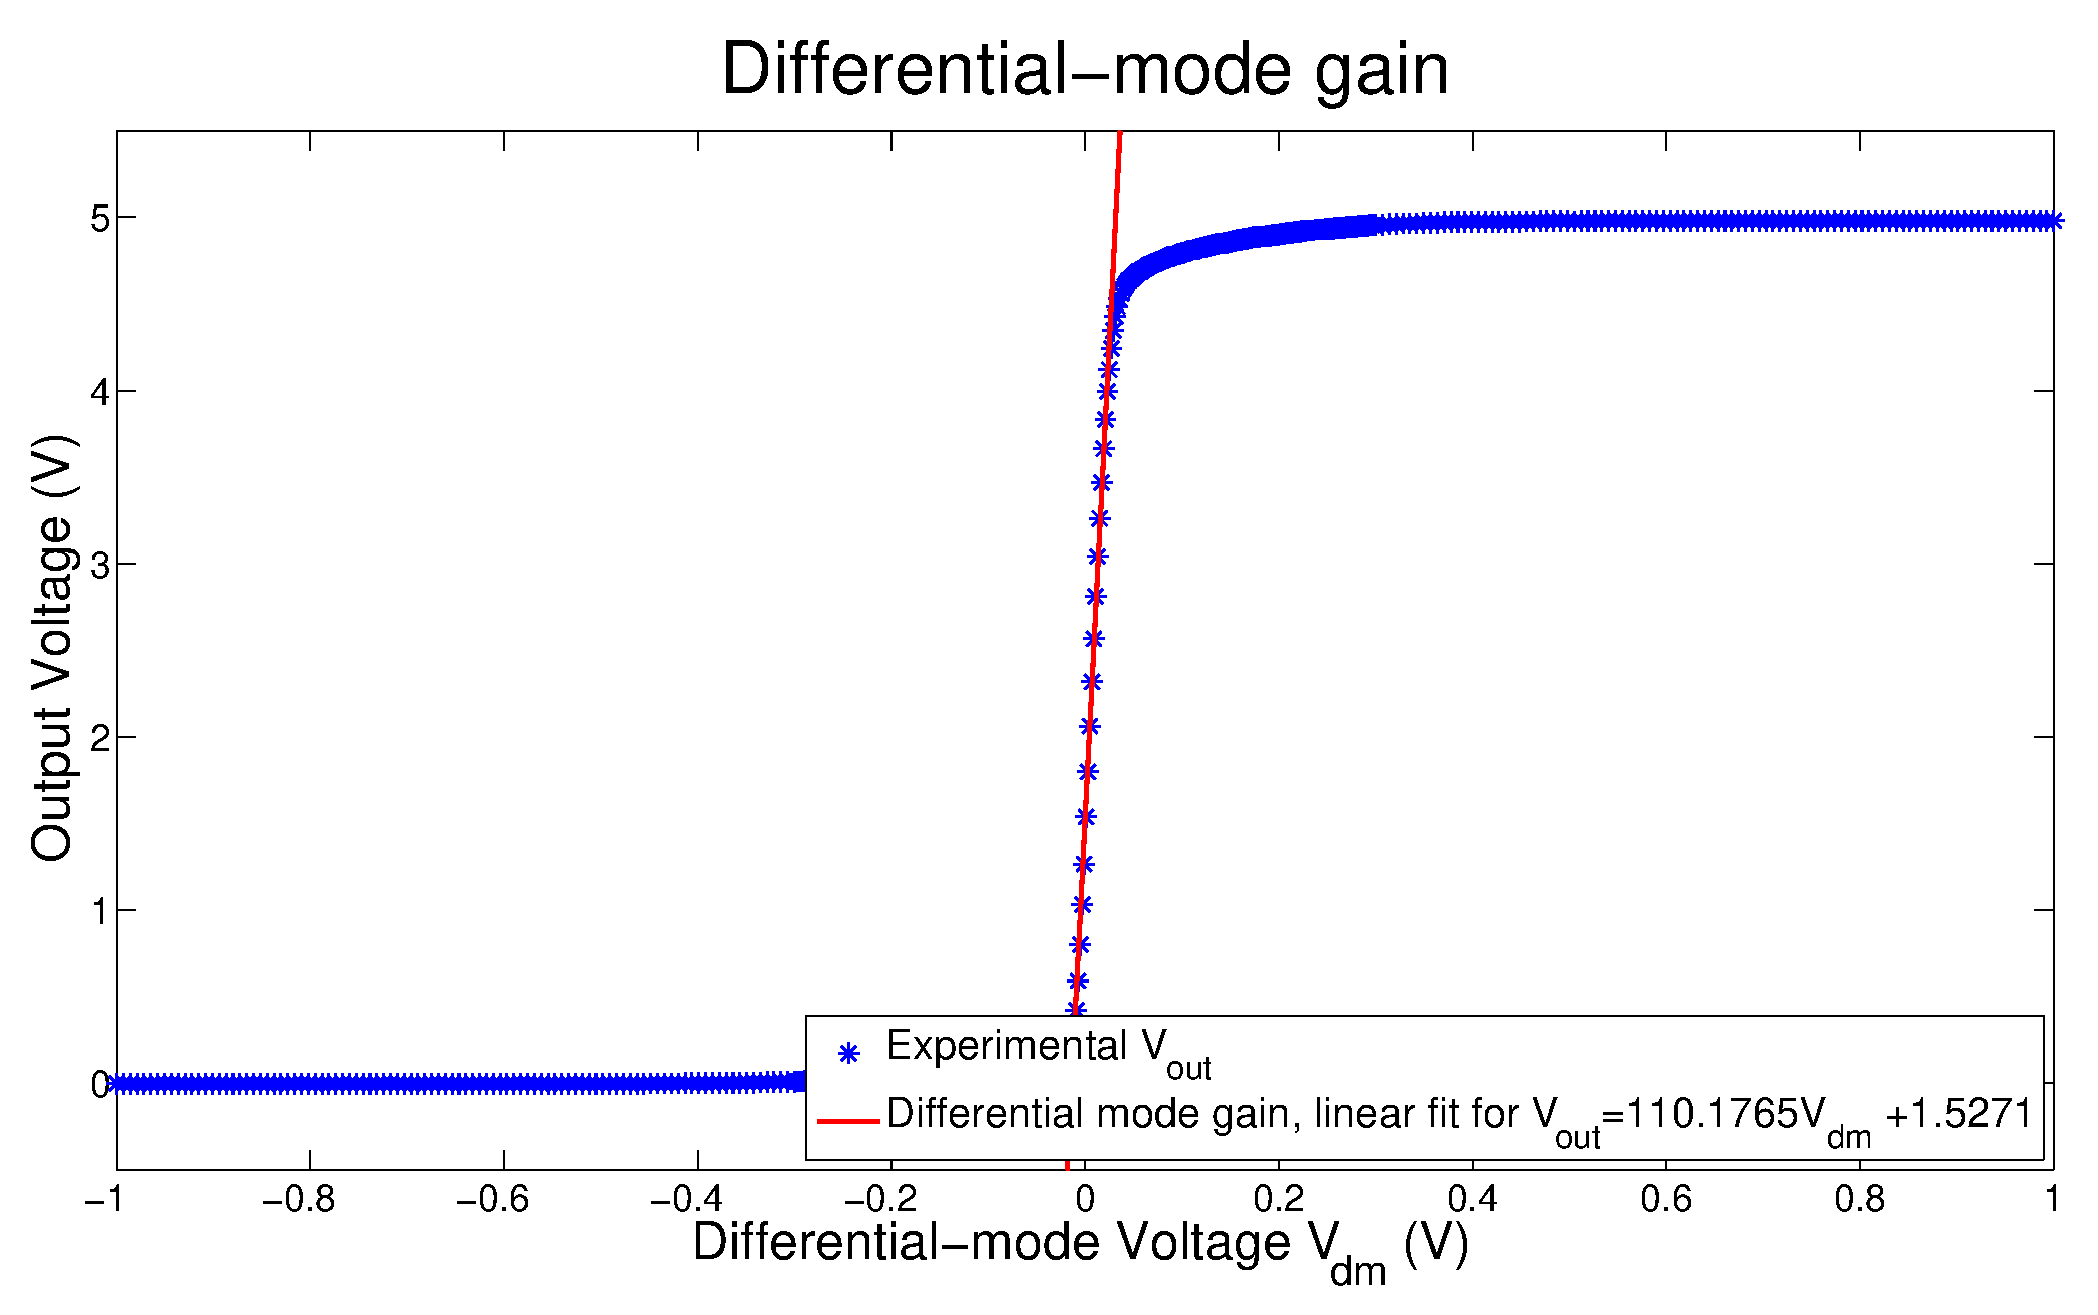
\includegraphics[width=\linewidth]{../Figures/Exp2P1.eps}
\caption{}
\label{fig:exp2p1}
\end{figure}

Next, we set the differential-mode input voltage to zero and measured the
current flowing into the output of the amplifer as we swept \Vout from one
rail to the other. We fit a straight line to the shallow part of this output
current–voltage characteristic in order to determine the incremental output
resistance of the circuit. The voltage transfer characteristic in this region
can be seen below in Figure \ref{fig:exp2p2}.
From the linear fit, we extracted an incremental output resistance of $489.6k\Omega$.




\begin{figure}[H]
\centering
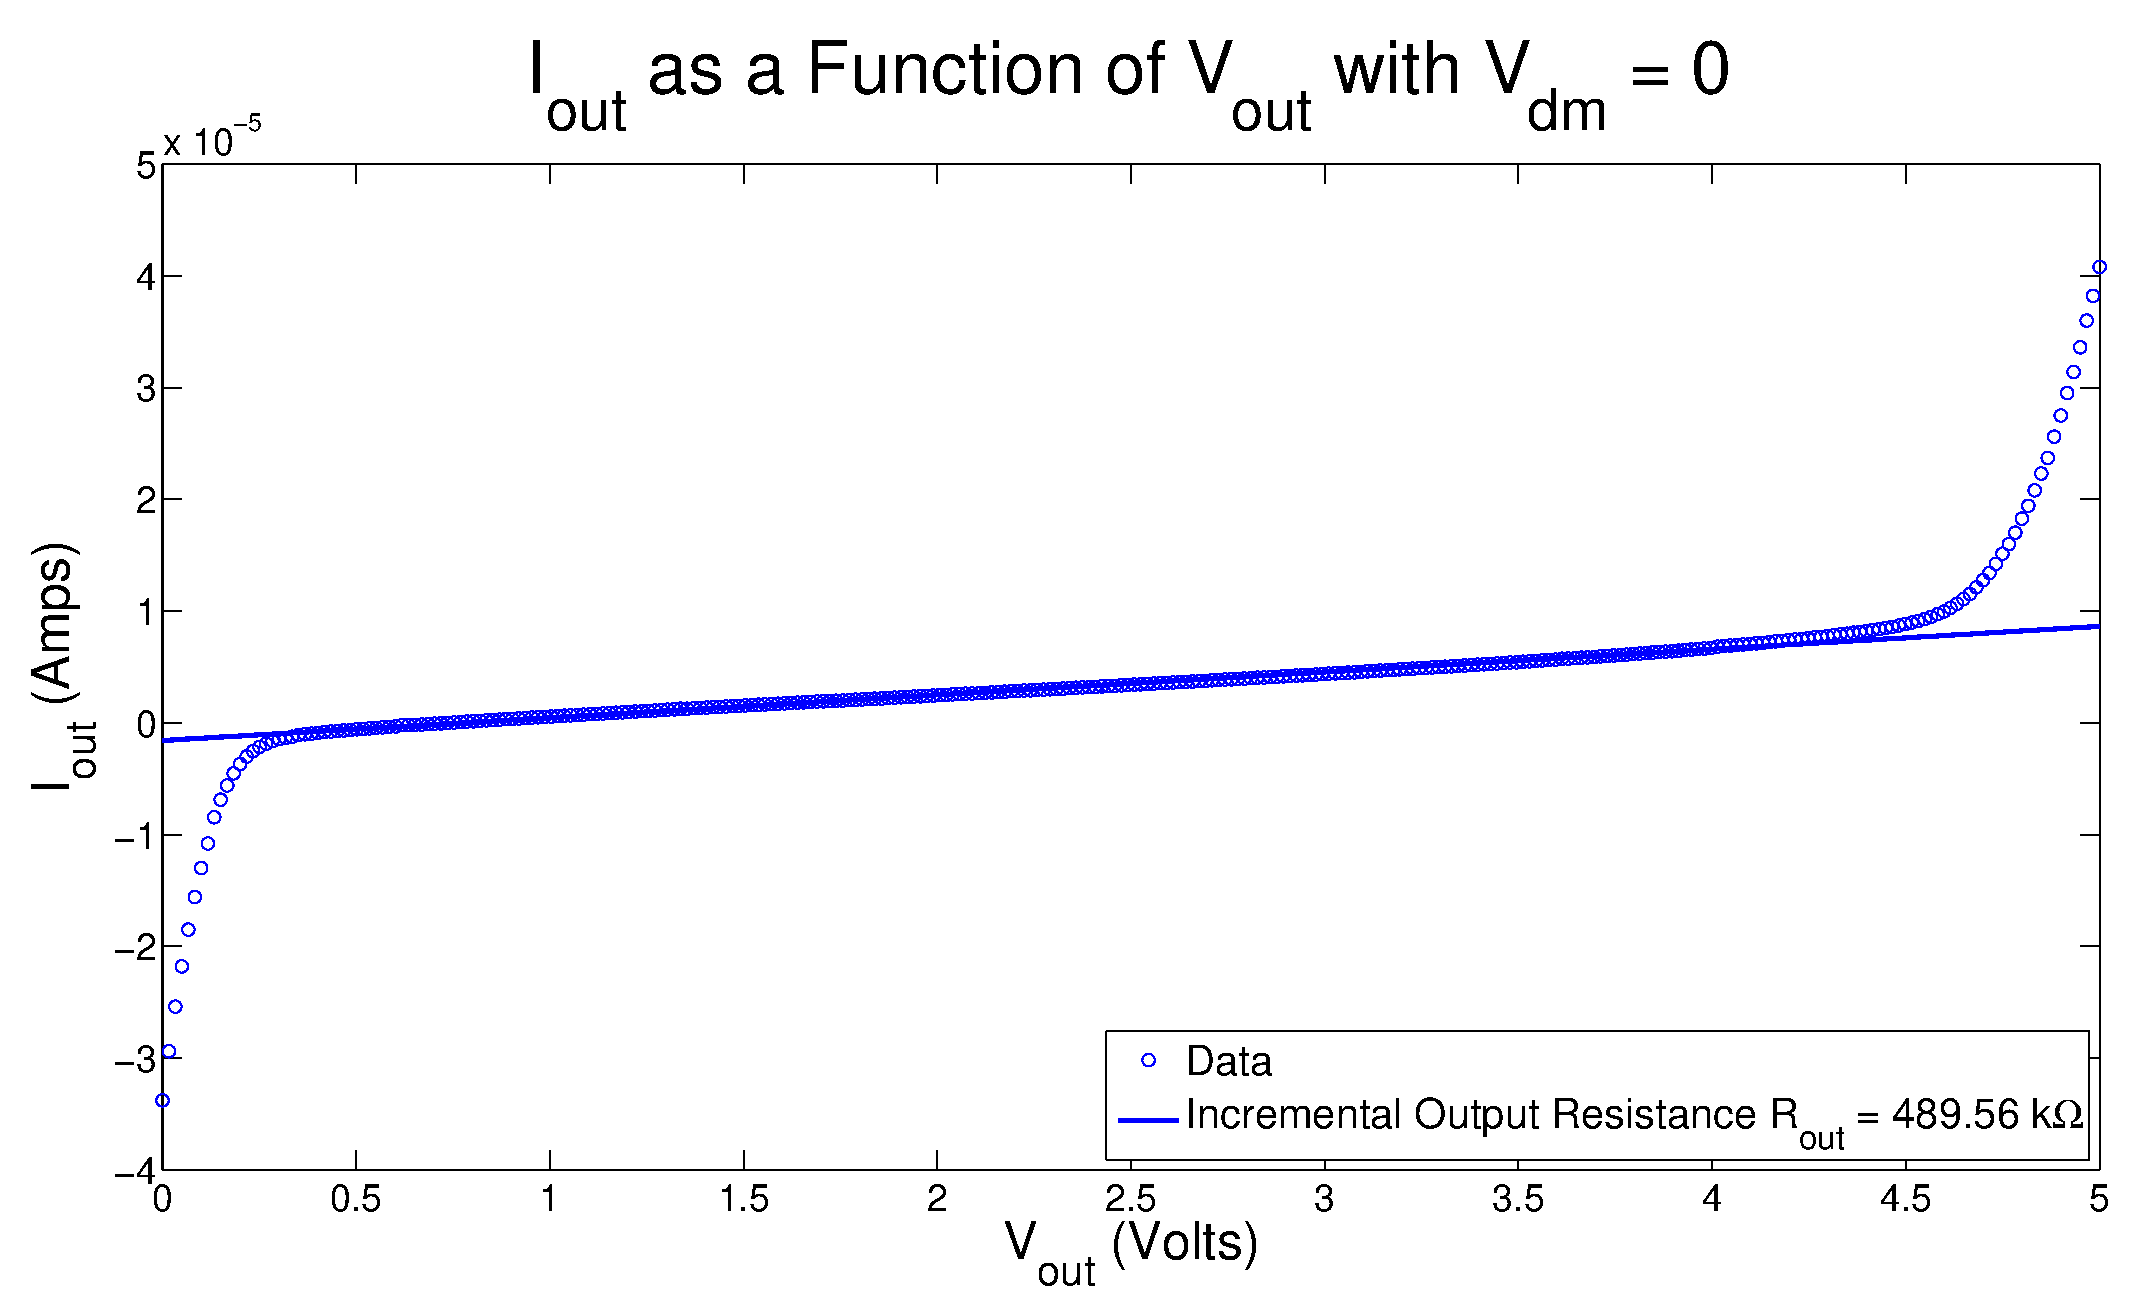
\includegraphics[width=\linewidth]{../Figures/Exp2P2.eps}
\caption{}
\label{fig:exp2p2}
\end{figure}

\begin{figure}[H]
\centering
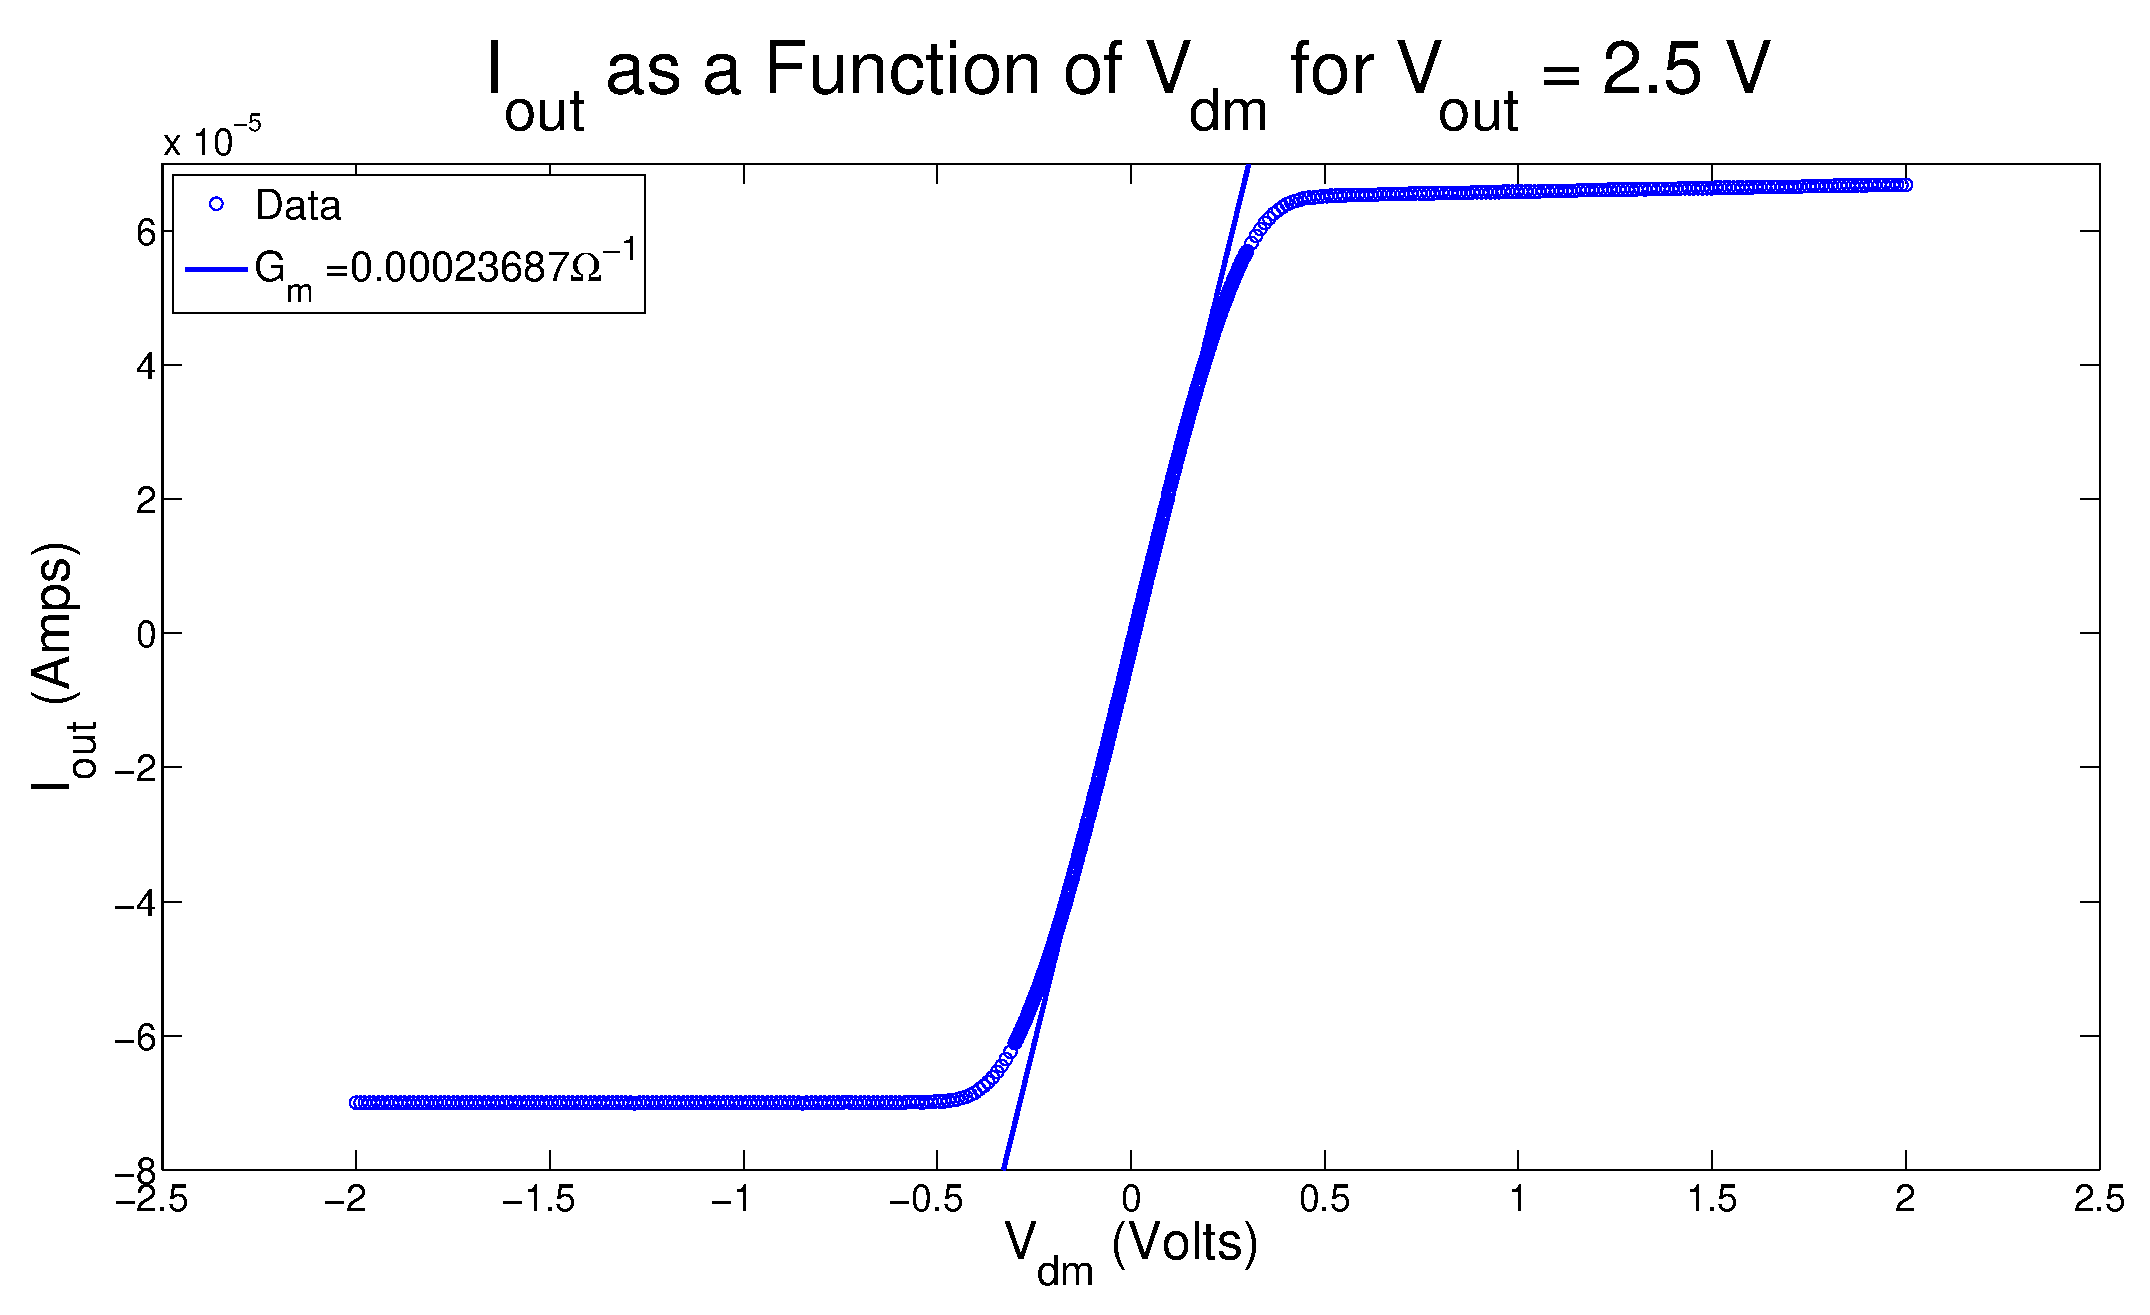
\includegraphics[width=\linewidth]{../Figures/Exp2P3.eps}
\caption{}
\label{fig:exp2p3}
\end{figure}